\documentclass[11pt]{article}
\usepackage[T1]{fontenc}
\usepackage[utf8]{inputenc}
\usepackage[a4paper,margin=1in]{geometry}
\usepackage{lmodern}
\usepackage{microtype}
\usepackage{amsmath,amssymb,amsthm,mathtools}
\usepackage{enumitem}
\usepackage{tikz}
\usetikzlibrary{arrows.meta,calc}
\usepackage{tikz-cd}
\usetikzlibrary{patterns}
\newcommand{\coxeterChamberOne}{%
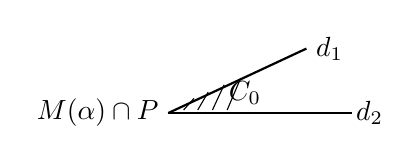
\begin{tikzpicture}[scale=.78,baseline=-.5ex]
  \coordinate (O) at (0,0);
  \draw[thick] (O)--(3.0,0);
  \draw[thick] (O)--(2.25,1.05);
  \draw[thin] (.25,.05)--(.42,.24);
  \draw[thin] (.48,.05)--(.65,.34);
  \draw[thin] (.72,.05)--(.91,.46);
  \draw[thin] (.96,.05)--(1.18,.57);
  \node at (1.25,.32){$C_0$};
  \node[right] at (2.9,0){$d_2$};
  \node[right] at (2.25,1.05){$d_1$};
  \node[left] at (0,0){$M(\alpha)\cap P$};
\end{tikzpicture}%
}
\newcommand{\coxeterChamberTwo}{%
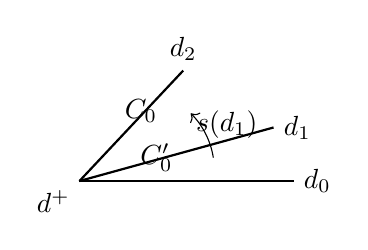
\begin{tikzpicture}[scale=.85,baseline=-.5ex]
  \coordinate (O) at (0,0);
  \draw[thick] (O)--(3.2,0) node[right]{$d_0$};
  \draw[thick] (O)--(2.9,.8) node[right]{$d_1$};
  \draw[thick] (O)--(1.55,1.65) node[above]{$d_2$};
  \node at (.92,1.05){$C_0$};
  \node at (1.15,.35){$C'_0$};
  \draw[->,thin] (2.0,.35) arc[start angle=9,end angle=45,radius=1.2];
  \node at (2.2,.85){$s(d_1)$};
  \node[below left] at (O){$d^+$};
\end{tikzpicture}%
}
\newcommand{\braidMoveSketch}{%
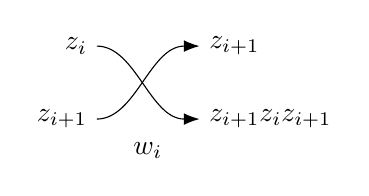
\begin{tikzpicture}[scale=.9,baseline=-.5ex]
  \draw[-{Latex[length=2mm]}] (0,.75) node[left]{$z_i$} .. controls (.55,.75) and (.75,-.28) .. (1.45,-.28) node[right]{$z_{i+1}z_i z_{i+1}$};
  \draw[-{Latex[length=2mm]}] (0,-.28) node[left]{$z_{i+1}$} .. controls (.55,-.28) and (.75,.75) .. (1.45,.75) node[right]{$z_{i+1}$};
  \node at (.72,-.72){$w_i$};
\end{tikzpicture}%
}

\setlength{\parindent}{0pt}
\setlength{\parskip}{0.55em}
\newcommand{\dd}{\,d}
\newcommand{\card}{\#}
\newcommand{\op}{\mathrm{op}}
\newcommand{\rank}{\mathrm{rang}}
\newcommand{\Stab}{\operatorname{Stab}}
\newcommand{\Cent}{\operatorname{Cent}}
\newcommand{\GL}{\operatorname{GL}}
\newcommand{\Id}{\operatorname{Id}}
\newcommand{\Int}{\operatorname{Int}}
\newcommand{\e}{\mathrm{e}}
\newtheoremstyle{plainfr}{.8em}{.8em}{\itshape}{}{}{.}{.5em}{}
\theoremstyle{plainfr}
\newtheorem*{theoreme}{Théorème}
\newtheorem*{lemme}{Lemme}
\newtheorem*{proposition}{Proposition}
\newtheorem*{corollaire}{Corollaire}
\newtheorem*{remarque}{Remarque}
\newenvironment{preuve}{\par\emph{Démonstration.}\ }{\hfill$\square$\par}
\begin{document}
\begin{flushright}
Bures-sur-Yvette, le 9 mars 1974
\end{flushright}

Cher Looijenga,

J'ai parlé de ton problème à Tits et Don Zagier, et ils me l'ont résolu.

\section*{1. Transformations de Coxeter}

\subsection*{1.1}
Soient $W$ un groupe de Coxeter fini, $D$ son diagramme de Dynkin, $V$ l'espace de sa représentation naturelle, et $R\subset W$ l'ensemble des réflexions. On appellera \emph{racine} un vecteur unitaire orthogonal à un hyperplan radiciel. Si $\alpha$ est une racine, on note
\[
 V^+(\alpha)=\{x\mid (x,\alpha)\geq 0\},\qquad M(\alpha)=\partial V^+(\alpha)
\]
le mur correspondant, et $z_\alpha\in R$ la réflexion par rapport à $M(\alpha)$. On suppose $D$ irréductible et $D\ne A_1$.

\subsection*{1.2}
Soit $c$ une transformation de Coxeter. Les faits suivants sont prouvés dans Bourbaki, \emph{Groupes et algèbres de Lie}, ch. V, §6, no. 2.

\begin{enumerate}[label=(\roman*),leftmargin=2.2em]
\item Soient $h$ l'ordre de $c$, et $P\subset V$ le plus grand sous-espace de $V$ où $c$ n'a que les valeurs propres $\exp(\pm 2\pi i/h)$. On a $\dim(P)=2$. On oriente $P$ pour que $c\vert_P$ soit une rotation d'amplitude $2\pi/h$.

\item Aucun mur ne contient $P$; les murs découpent sur $P$ un système d'hyperplans radiciels de type $I_2(h)$.

\item Les murs de $V$ contenant un même mur $d$ de $P$ sont deux à deux orthogonaux. On note $s(d)$ l'involution produit des réflexions correspondantes.

\item Soient $C_0$ une chambre de $P$, $C$ l'unique chambre de $V$ la contenant, $d_1^+$ et $d_2^+$ les demi-droites limitant $C_0$, prises dans le sens direct, et $d_1,d_2$ les droites correspondantes. Alors les murs de $C$ sont ceux contenant $d_1$ ou $d_2$, et
\[
 c=s(d_2)s(d_1).
\]
De plus, $s(d_i)$ stabilise $P$, sa restriction à $P$ est la réflexion par rapport à $d_i$, et $c\vert_P$ est donc une transformation de Coxeter de $P$.
\end{enumerate}

Soient $c\in W$ un élément de Coxeter, et $\alpha$ une racine.

\begin{corollaire}[1.3]
\begin{enumerate}[label=(\roman*),leftmargin=2.2em]
\item Avec les notations de 1.2(iv), le groupe diédral $W'$ engendré par $s(d_1)$ et $s(d_2)$ est le stabilisateur de $P$. C'est aussi le stabilisateur de $\{c,c^{-1}\}$. $W'$ agit fidèlement sur $P$, et sa restriction à $P$ est le groupe de Weyl de $P$. Le centralisateur de $c$ est le sous-groupe $\langle c\rangle$ engendré par $c$.

\item Il existe une chambre $C$, dont $\alpha$ soit racine simple, et une énumération $(\alpha_1,\ldots,\alpha_\ell)$ des racines simples de $C$, avec $\alpha=\alpha_1$, telle que
\[
 c=z_{\alpha_1}\cdots z_{\alpha_\ell}.
\]

\item Pour $C$ comme en (ii), la droite $d$ intersection des murs $M(\alpha_i)$, $i\ne 1$, est le sous-espace de $V$ fixé par $z_\alpha c$. Elle ne dépend donc pas de $C$. Le sous-groupe $W_d$ de $W$ qui fixe $d$ est de Coxeter, engendré par les $z_{\alpha_i}$, $i\ne 1$; sa représentation naturelle est sur $V/d$, et $z_\alpha c\in W_d$ est une transformation de Coxeter de $W_d$.

\item Le sommet de $D$ correspondant au mur $M(\alpha)$ de $C$, $C$ comme en (ii), est indépendant de $C$. On le note $\bar\alpha$.

\item $\langle c\rangle$ agit librement sur l'ensemble des racines. Deux racines sont dans la même orbite si et seulement si elles ont même image dans $D$.

\item Soient $C_0$ et $C$ comme en 1.2(iv). Pour chaque mur $M$ de $C$, soit $\alpha=\alpha(M)$ la racine telle que $M=M(\alpha)$ et que $V^+(\alpha)$ contienne, respectivement ne contienne pas, $C$ selon que $M$ passe par $d_2$, respectivement par $d_1$. Alors
\[
 \{\alpha(M)\mid M\text{ mur de }C\}
\]
est une section de l'ensemble des orbites de $\langle c\rangle$, et $\bar\alpha(M)$ est la classe dans $D$ du mur $M$ de $C$.
\end{enumerate}
\end{corollaire}

\begin{preuve}
Pour (i), $W'$ stabilise $\{c,c^{-1}\}$ car $s(d_i)c s(d_i)^{-1}=c^{-1}$. Réciproquement, $\{c,c^{-1}\}$ détermine $P$; le stabilisateur de $\{c,c^{-1}\}$ stabilise donc $P$. Un élément $w\in W$ qui stabilise une chambre $C_0$ de $P$ est l'identité, car $C_0$ est contenue dans une seule chambre. Puisque $W'$ est transitif sur les chambres de $P$, c'est le stabilisateur de $P$ tout entier. Enfin, $\langle c\rangle$ est le centralisateur de $c$ dans $W'$, donc dans $W$.

Pour (ii), on prend la chambre $C_0$ de $P$ de mur $M(\alpha)\cap P$, telle que, avec les notations de 1.2(iv), $M(\alpha)\cap P=d_2$ et $V^+(\alpha)\supset C_0$. Puisque $c=s(d_2)s(d_1)$, ce choix convient.
\[
\coxeterChamberOne
\]

Pour (iii), on a $z_\alpha c=z_{\alpha_2}\cdots z_{\alpha_\ell}$; la première assertion en résulte facilement. Que $z_\alpha c$ soit de Coxeter se voit en prenant $C$ comme en (ii).

Pour (iv), on va vérifier que $\bar\alpha$ ne dépend que de $\alpha$ et de $d$. Si $C'$ et $C''$ sont deux chambres dont $\alpha$ est racine simple, et telles que la demi-droite opposée au mur $M(\alpha)$ soit $d^+=d\cap V^+(\alpha)$, il existe $w\in W_d$ envoyant $C'$ sur $C''$; les chambres contenant $d^+$ correspondent biunivoquement à celles de $V/d$. Puisque $w$ respecte $d$, il respecte $M(\alpha)$, et (iv) en résulte.

En écrivant $c=s(d_2)s(d_1)$, on voit aussitôt, pour $M$ passant par $d_2$, que $\bar\alpha(M)$ est la classe du mur $M$ de $C$. Soit $C_0'=s(d_1)C_0$, d'où $C'=s(d_1)C$. On obtient de même le cas des murs passant par $d_1$. Il est clair que les $\bar\alpha(M)$ forment une section de l'ensemble des orbites de $\langle c\rangle$ dans l'ensemble des racines, et que l'action de $\langle c\rangle$ est libre. Comme $c^{-1}\alpha$ se transporte de même, (v) et (vi) s'en déduisent.
\[
\coxeterChamberTwo
\]
\end{preuve}

\begin{remarque}[1.4]
Ne supposons plus $D$ irréductible, ni $D\ne A_1$. Les assertions (ii), (iii), (iv) valent encore. La deuxième partie de (v) vaut en remplaçant $\langle c\rangle$ par le centralisateur de $c$. On notera $h(D)$ l'ordre de ce centralisateur; ainsi
\[
 h\Bigl(\coprod D_i\Bigr)=\prod h(D_i).
\]
\end{remarque}

\begin{corollaire}[1.5]
Soient $W$ un groupe de Coxeter fini et $c\in W$ un élément de Coxeter. Soit $\Xi_c$ l'ensemble des suites de $\ell$ racines $\alpha_1,\ldots,\alpha_\ell$, et soit $\Xi'_c$ l'ensemble des suites de $\ell$ réflexions $z_1,\ldots,z_\ell$, $\ell=\rank W$, telles que
\[
 z_{\alpha_1}\cdots z_{\alpha_\ell}=c,\qquad z_1\cdots z_\ell=c.
\]
Les nombres
\[
 F(D)=\card\Xi_c,\qquad F'(D)=\card\Xi'_c
\]
ne dépendent que de $D$, et vérifient $F(D)=2^\ell F'(D)$. On a, pour $D$ irréductible,
\[
 F(D)=h(D)\sum_{i\in D}F(D-\{i\}),
\]
d'où
\[
 F'(D)=\frac{h(D)}{2}\sum_{i\in D}F'(D-\{i\}).
\]
D'après 1.3(ii), on a en effet
\[
 F(D)=\sum_{\alpha\;\mathrm{racine}}F(D-\{\bar\alpha\}),
\]
et on applique 1.3(v), complété par 1.4.
\end{corollaire}

\begin{remarque}[1.6]
On a $F(\varnothing)=F'(\varnothing)=1$. Pour des diagrammes $D_i$ de rangs $\ell_i$, et $D=\coprod D_i$, $\ell=\sum\ell_i$, on a
\[
 F(D)=\frac{\ell!}{\prod\ell_i!}\prod_i F(D_i),
\]
et de même pour $F'$.
\end{remarque}

\begin{remarque}[1.7]
Pour $c$ fixé, on a défini une application $\alpha\mapsto\bar\alpha$ de l'ensemble des racines dans $D$. On a $\overline{-\alpha}$ égal au transformé de $\bar\alpha$ par l'involution d'opposition. Dès lors, notant $D'$ le quotient de $D$ par l'involution d'opposition, $\alpha\mapsto\bar\alpha$ passe au quotient et définit une application $z\mapsto \bar z:R\to D'$.
\end{remarque}

\section*{2. Action du groupe des tresses}

Soient $W$ un groupe de Coxeter fini, $D$ son diagramme de Dynkin, $D'$ le quotient de $D$ par l'involution d'opposition, $\ell$ le rang de $W$, $c$ une transformation de Coxeter et $\Xi'_c$ comme en 1.5. Soit $B_\ell$ le groupe de tresses à $\ell$ brins, de générateurs canoniques $(w_i)_{1\le i\le \ell-1}$. On le fait agir sur $\Xi'_c$ par
\[
 w_i:(z_1,\ldots,z_\ell)\longmapsto (z_1,\ldots,z_{i-1},z_{i+1},z_{i+1}z_i z_{i+1},z_{i+2},\ldots,z_\ell).
\]
\[
\braidMoveSketch
\]

\begin{theoreme}[2.1]
$B_\ell$ agit transitivement sur $\Xi'_c$.
\end{theoreme}

\begin{preuve}
On procède par récurrence sur $\ell$. Si $D$ est somme disjointe de diagrammes $D_i$, et si le théorème est vrai pour les $D_i$, il l'est pour $D$. Ceci nous ramène à supposer $D$ irréductible. Les cas $D=\varnothing$ ou $A_1$ sont triviaux.

\begin{lemme}[2.1.1]
Soient $\sigma'=(z'_1,\ldots,z'_\ell)$ et $\sigma''=(z''_1,\ldots,z''_\ell)$ dans $\Xi'_c$. Si $z'_1=z''_1$, alors $\sigma'$ et $\sigma''$ sont dans la même orbite de $B_\ell$.
\end{lemme}

Soit $d$ le sous-espace de $V$ fixé par $z'_1c$. On applique l'hypothèse de récurrence à $W_d$ et à $\Xi'_{z'_1c}$, conformément à 1.3(iii).

Disons que deux racines $\alpha$ et $\beta$ sont équivalentes s'il existe $\sigma'=(z'_1,\ldots,z'_\ell)$ et $\sigma''=(z''_1,\ldots,z''_\ell)$ dans $\Xi'_c$, conjugués sous $B_\ell$, tels que $z'_1=z_\alpha$ et $z''_1=z_\beta$. Il reste à prouver que deux racines sont toujours équivalentes.

\begin{enumerate}[label=(\alph*),leftmargin=2.2em]
\item $\alpha$ et $c^{-1}\alpha$ sont équivalentes. On prend $\sigma=(z_\alpha,z_2,\ldots,z_\ell)$ dans $\Xi'_c$; alors
\[
 w_1\cdots w_{\ell-2}w_{\ell-1}w_{\ell-2}\cdots w_1(\sigma)=(c^{-1}z_\alpha c,\ldots).
\]

\item $\alpha$ et $-\alpha$ sont équivalentes, puisque $z_\alpha=z_{-\alpha}$.
\end{enumerate}

D'après 1.3(v) et 1.7, il existe donc une relation d'équivalence sur $D'$ telle que $\alpha\sim\beta$ si et seulement si $\bar\alpha$ et $\bar\beta$ ont des images équivalentes sur $D'$. Puisque $W$ agit trivialement sur $D'$, cette équivalence ne dépend pas du choix de $c$. On note encore $\sim$ l'équivalence image réciproque sur $D$.

\begin{enumerate}[label=(\alph*),leftmargin=2.2em,start=3]
\item Pour $i,j$ deux sommets non liés de $D$, on a $i\sim j$. On prend $c=z_i z_j\cdots$, produit de réflexions fondamentales. Alors
\[
 w_1(z_i,z_j,\ldots)=(z_j,z_i,\ldots),
\]
et $\bar z_i=i$, $\bar z_j=j$.

\item Pour $i,j$ comme ci-dessous, avec $i$ pendant, on a $i\sim j$.
\[
\begin{tikzpicture}[baseline=-.5ex,scale=.7]
\draw (0,0)--(1.2,0)--(2.3,0);
\fill (0,0) circle (2pt) node[below]{$i$};
\fill (1.2,0) circle (2pt) node[below]{$j$};
\fill (2.3,0) circle (1.5pt);
\draw[dotted] (2.45,0)--(3.2,0);
\end{tikzpicture}
\]
On prend $c=z_jz_i\cdots$, produit de réflexions fondamentales. Alors
\[
 w_1(z_j,z_i,\ldots)=(z_i,z_i z_j z_i,\ldots),
\]
où $z_i z_j z_i$ est la réflexion fondamentale pour la chambre $z_iC$, et $\bar z_j=j$, $\bar z_i=i$.
\end{enumerate}

De (c) et (d) résulte l'équivalence de tous les sommets, et le théorème.
\end{preuve}

\section*{3. Calcul de $F'(D)$}

\begin{corollaire}[3.1]
\[
 F'(A_\ell)=(\ell+1)^{\ell-1}.
\]
Dans ce cas, tu as en effet démontré directement ta conjecture; tandis que, par 2.1, $\Xi'_c$ ne forme qu'une orbite sous $B_\ell$, et on applique ton calcul de l'indice.

C'est aussi équivalent à la formule que tu indiques sur les arbres: pour qu'un produit de $\ell$ transpositions dans un ensemble à $\ell+1$ éléments soit un $(\ell+1)$-cycle, il faut et suffit que le graphe obtenu en liant les points qui figurent dans ces transpositions soit un arbre. Puisqu'il y a $\ell!$ $(\ell+1)$-cycles et $\ell!$ ordres totaux sur un arbre donné, on a
\[
 F'(A_\ell)=\card\{\text{arbres de support un ensemble à }(\ell+1)\text{ éléments donné}\}.
\]
\end{corollaire}

\subsection*{3.2}
Le corollaire 1.5 fournit
\[
F'(A_\ell)=\frac{\ell+1}{2}
\sum_{\substack{i+j=\ell-1\\ i,j\ge0}}
\frac{(\ell-1)!}{i!j!}\,F'(A_i)F'(A_j),
\]
soit
\[
2\ell\frac{F'(A_\ell)}{\ell!}=(\ell+1)\sum_{i+j=\ell-1}\frac{F'(A_i)}{i!}\frac{F'(A_j)}{j!}.
\]
En termes de la série génératrice
\[
 a(t)=\sum_{i=0}^{\infty}\frac{F'(A_i)}{i!}t^{i+1},
\]
ceci s'écrit
\[
2t\,\partial_t\left(\frac{a}{t}\right)=\partial_t(a^2),
\]
c'est-à-dire
\[
 \dd a-a\frac{\dd t}{t}=a\,\dd a,
\]
soit
\[
 \frac{\dd a}{a}-\dd a=\frac{\dd t}{t}.
\]
Puisque $a'(0)=1$, on obtient
\[
 a\,e^{-a}=t.
\]

\begin{corollaire}[3.3]
\[
 F'(B_\ell)=\ell^\ell.
\]
Ici, $W$ est le sous-groupe de $\GL(\ell,\mathbb R)$ qui respecte une tribu $\{\pm\varepsilon_i\}$; on a $|W|=2^\ell\ell!$, $h=2\ell$, par exemple
\[
 c:\varepsilon_1\mapsto\varepsilon_2\mapsto\cdots\mapsto\varepsilon_\ell\mapsto-\varepsilon_1,
\]
et le nombre d'éléments de Coxeter est $2^{\ell-1}(\ell-1)!$.

Pour qu'un produit de $\ell$ réflexions soit de Coxeter, il faut et suffit que:
\begin{enumerate}[label=(\alph*),leftmargin=2.2em]
\item une et une seule d'entre elles soit du type $(\varepsilon_i\mapsto-\varepsilon_i,\;\varepsilon_j\text{ fixe})$;
\item le graphe suivant soit un arbre: on met une arête pour chacune des réflexions qui joint $i$ à $j$ par une réflexion $\varepsilon_i\mapsto\pm\varepsilon_j$.
\end{enumerate}
Dès lors, le nombre de suites de $\ell$ réflexions dont le produit est de Coxeter est
\[
 \ell^{\ell-2}(\ell-1)!\,2^{\ell-1}\ell^2,
\]
et le cardinal de chaque $\Xi'_c$ est donc
\[
 \frac{\ell^{\ell-2}(\ell-1)!\,2^{\ell-1}\ell^2}{2^{\ell-1}(\ell-1)!}=\ell^\ell.
\]
\end{corollaire}

\subsection*{3.4}
Le corollaire 1.5 fournit, avec $B_0=\varnothing$ et $B_1=A_1$, pour $\ell\ge1$,
\[
 F'(B_\ell)=\ell\sum_{i+j=\ell-1}\frac{(\ell-1)!}{i!j!}\,F'(A_i)F'(B_j),
\]
soit
\[
 \frac{F'(B_\ell)}{\ell!}=\sum_{i+j=\ell-1}\frac{F'(A_i)}{i!}\frac{F'(B_j)}{j!}.
\]
En termes de la série génératrice
\[
 b(t)=\sum_{i=0}^\infty\frac{F'(B_i)}{i!}t^i,
\]
ceci s'écrit
\[
 b(t)=a(t)b(t)+1,
\]
c'est-à-dire
\[
 b(t)=\frac1{1-a(t)}.
\]

\begin{corollaire}[3.5]
\[
 F'(D_\ell)=2(\ell-1)^\ell\qquad (\ell\ge2).
\]
Soit la série génératrice
\[
 d(t)=1+\sum_\ell\frac{F'(D_\ell)}{2\ell!}t^\ell.
\]
Le corollaire 1.5 fournit
\[
F'(D_\ell)=(\ell-1)\left[
\sum_{\substack{i+j=\ell-1\\ j\ge2}}
\frac{(\ell-1)!}{i!j!}F'(A_i)F'(D_j)+2F'(A_{\ell-1})\right],
\]
donc
\[
\ell\frac{F'(D_\ell)}{2\ell!}=(\ell-1)\left[
\sum_{\substack{i+j=\ell-1\\ j\ge2}}
\frac{F'(A_i)}{i!}\frac{F'(D_j)}{2j!}
+\frac{F'(A_{\ell-1})}{(\ell-1)!}\right].
\]
En multipliant par $t^{\ell-1}$ et en prenant la somme, cela donne
\[
 \partial_t d=t\partial_t\left(\frac{ad}{t}\right),
\]
soit
\[
\partial_t d=\partial_t d\cdot a+d\cdot t\partial_t\left(\frac{a}{t}\right),\qquad
 t\partial_t\left(\frac{a}{t}\right)=a\partial_t a.
\]
Ainsi
\[
 \partial_t d(1-a)=d\,a\,\partial_t a,
\]
\[
 \frac{\partial_t d}{d}=\frac{a\partial_t a}{1-a}=\partial_t\{-a-\log(1-a)\},
\]
et
\[
 d=\frac{e^{-a}}{1-a}.
\]
Comme $ae^{-a}=t$, on obtient encore
\[
 d=\frac{t}{a(1-a)},\qquad \frac{ad}{t}=b.
\]
Reportant dans l'équation différentielle ci-dessus, on trouve
\[
 \partial_t d=t\partial_t b,
\]
ce qui est le corollaire.
\end{corollaire}

J'ai aussi vérifié que
\[
 F'(E_6)=2^9 3^4,
 \qquad F'(E_7)=2\cdot 3^{12},
 \qquad F'(E_8)=2\cdot 3^5\cdot 5^7.
\]
On a prouvé ta conjecture.

\section*{4. Compléments}

\subsection*{4.1}
Le résultat suivant précise 1.3(ii).

Soient $W$ un groupe de Coxeter fini de diagramme de Dynkin $D$ irréductible. Soient $\leq$ un ordre total sur $D$, et $\alpha$ une racine. Pour chaque chambre $C$ dont $\alpha$ est racine simple, soient $\alpha_1,\ldots,\alpha_\ell$ les racines simples associées à $C$, dans l'ordre $\leq$, et soit
\[
 c(C)=z_\alpha z_{\alpha_1}\cdots \widehat{z_\alpha}\cdots z_{\alpha_\ell},
\]
le produit des $z_{\alpha_i}$ dans l'ordre $\leq$, sauf que $z_\alpha$ est mis devant.

\begin{proposition}[4.2]
L'application
\[
 C\longmapsto c(C)
\]
de l'ensemble des chambres dont $\alpha$ est racine simple dans l'ensemble des transformations de Coxeter est bijective.
\end{proposition}

L'injectivité se prouve comme 1.3(iv). Avec les notations de loc. cit., soit $w\in W_d$ envoyant $C'$ sur $C''$. Il respecte $\alpha$ et l'ordre des murs, donc respecte $c(C')=c(C'')$. Puisque $w$ centralise une transformation de Coxeter et fixe une racine, $w=1$, d'après 1.3(i) et (v).

Il reste à compter. Il y a $|W|/h$ transformations de Coxeter, par 1.3(i). Si $\ell_\alpha$ est le nombre de sommets du diagramme de Dynkin correspondant à des racines conjuguées à $\alpha$, alors $\alpha$ a $\ell_\alpha h$ conjuguées sous $W$, par 1.3(v). Le nombre de couples
\[
(\text{racine }\beta\text{ conjuguée à }\alpha,
\text{ chambre dont }\beta\text{ est racine simple})
\]
est $|W|\ell_\alpha$; le nombre de chambres dont $\alpha$ est racine simple est donc $|W|/h$.

Bien à toi,

\hfill P. Deligne

\end{document}
